\documentclass{beamer}
\usepackage[utf8]{inputenc}
\usepackage{hyperref}

\usepackage{tikz}

\usepackage{latexsym,xcolor,multicol,booktabs,calligra}
\usepackage{amsmath,amssymb,BOONDOX-cal,bm}	
\usepackage{graphicx,pstricks,stackengine} 
\usepackage{libertinus}
\usepackage{amssymb}
\usepackage{pgfplots}
\usepackage{tikz}
\usepackage{xcolor}
\usepackage{array}
\usetikzlibrary{positioning}

\usepackage{etoolbox}
\makeatletter
\newcommand{\noframenumbering}{%
  \beamer@noframenumberingtrue%
}
\makeatother

\usepackage[T1]{fontenc}

\title{Macroeconometrics\\
7 - (Panel VAR), Cointegration, \& Dynamic Factor Models}
\author{Camille Souffron\\
Ecole Normale Supérieure \& Paris School of Economics\\
\textcolor{blue}{\href{mailto:camille.souffron@ens.psl.eu}{camille.souffron@ens.psl.eu}}}
\institute{\normalsize M2 EPOG JM}
\date{Fall 2026}

\usetheme{Singapore}

\def\cmd#1{\texttt{\color{red}\footnotesize $\backslash$#1}}
\def\env#1{\texttt{\color{RoyalBlue}\footnotesize #1}}

\newtheorem{thm}{Theorem}[theorem]
\setbeamertemplate{footline}[frame number]

\begin{document}

\begin{frame} % <-- no [plain] here!
    \titlepage % This keeps the theme style
    \begin{center}
        
\includegraphics[width=0.5\textwidth]{logos.png}
    \end{center}
\end{frame}



\addtocounter{framenumber}{-1}


\section{Panel VAR}

\begin{frame}{A Note on Panel VAR}
\small

\textbf{Panel VAR (PVAR):} a VAR framework for \textit{panel data}, modelling dynamic interactions \textbf{\emph{within}} each unit while exploiting repeated observations \textbf{\emph{across}} units. E.g.\ credit, capital and risk for 100 banks over 10 years. Or output, inflation and employment for 20 countries or sectors. 

\[
y_{i,t} = a_i + \sum_{\ell=1}^p A_{i\ell} y_{i,t-\ell} + u_{i,t},
\qquad i=1,\dots,N.
\]

\begin{itemize}
  \item $y_{i,t}$ is a $k$-vector of endogenous variables for unit $i$.
  \item $a_i$ captures \textbf{unit-specific fixed effects (FE).}
  \item The model describes \textbf{domestic / within-unit dynamics}: how variables of unit $i$
  affect each other over time.
  \item PVARs are useful when one wants to learn common or average dynamic patterns
  from many comparable units.
  \item The central modelling choice is \textbf{how much heterogeneity to allow} in
  $A_{i\ell}$ across units.
\end{itemize}
Should the slope matrices be pooled, partially pooled, or estimated separately?


\end{frame}

%======================================================
\begin{frame}{PVAR: Pooled}
%======================================================
\footnotesize

\textbf{Strategy 1 - Pooled PVAR} \quad\textit{(units are homogeneous)}

\smallskip

\begin{itemize}
    \item \textit{Assumption:} same slopes across units $A_{i\ell}=A_\ell$ for all $i$; only intercepts $a_i$ differ.

\item \textit{Estimation challenge:} to remove $a_i$, demean or first-difference. But the PVAR is dynamic: $y_{i,t-1}$ appears on the RHS \emph{and} in the demeaned LHS $\Rightarrow$ \textbf{Nickell (1981) bias}: the within-group estimator is \textbf{inconsistent} with fixed $T$ (bias $\sim -\frac{1+\rho}{T}$, does not vanish as $N\to\infty$).\footnote{\scriptsize
Intuition in the AR(1) case $y_{i,t}$:
first-differencing removes $a_i$ but gives
$\Delta y_{i,t}$ $=\rho \Delta y_{i,t-1}+\Delta u_{i,t}$, where
$\Delta u_{i,t}=u_{i,t}-u_{i,t-1}$. Since $\Delta y_{i,t-1}$ $=y_{i,t-1}-y_{i,t-2}$
contains $u_{i,t-1}$, it is correlated with $-u_{i,t-1}$ in $\Delta u_{i,t}$.
Thus OLS/within estimation is biased even if $u_{i,t}$ is serially uncorrelated.
The bias (order $1/T$) does not vanish when $N\to\infty$ with fixed $T$.}

\item \textit{Fix - General Method of Moment  (GMM) estimation (Arellano \& Bond, 1991; Blundell \& Bond, 1998):}
\begin{itemize}
\footnotesize
  \item First-difference the equation to remove $a_i$, then instrument $\Delta y_{i,t-1}$ with \emph{levels} $y_{i,t-2}, y_{i,t-3},\dots$ (valid if $u_{i,t}$ is serially uncorrelated).
  \item \textbf{System-GMM} adds the levels equation (instrumented with differences) for better finite-$T$ precision.
\end{itemize}

\item \textit{Use case:} similar-sized banks, firms in same sector, regions under same institutional framework.


\item \textbf{But inconsistent if slopes truly differ} (Pesaran \& Smith, 1995).
\end{itemize}

\end{frame}

%======================================================
\begin{frame}{PVAR: Hierarchical}
%======================================================
\small

\textbf{Strategy 2 - Hierarchical Panel VAR} \quad\textit{(units heterogeneous but structurally related)}\footnote{\scriptsize The natural implementation is \textbf{Bayesian hierarchical}: place a common prior $A_{i\ell}\sim\mathcal{N}(\bar A_\ell,\Sigma_A)$, estimate via MCMC/Gibbs. This gives \emph{partial pooling}: unit estimates shrink toward the group mean except if strong difference (disciplined by data) (Canova \& Ciccarelli, 2004; Jaroci\'nski, 2010).}


\smallskip

\begin{itemize}
\item \textit{Assumption:} each unit has \emph{its own} slope $A_{i\ell}$, but units share a \textbf{common group structure} (e.g.\ countries in the same currency union, banks in the same regulatory tier, sectors in the same country).

\item \textit{Estimation:} estimate unit-specific VARs \emph{jointly}, imposing that slopes are drawn from a common distribution. The group-level parameters $(\bar A_\ell, \Sigma_A)$ are estimated alongside unit-level ones 

\item $\Rightarrow$ \textbf{Partial pooling}: countries with little data are shrunk toward the global mean, while countries with abundant information remain close to their own estimates.

\item \textit{Use case:} heterogeneous countries/sectors with \emph{small $T$}, where estimating fully separate VARs would be too noisy.

\end{itemize}
\end{frame}


%======================================================
\begin{frame}{PVAR: Mean Group}
%======================================================
\footnotesize

\textbf{Strategy 3 - Mean Group (MG) estimator} (Pesaran \& Smith, 1995) \quad\textit{(units fully heterogeneous)}

\smallskip

\begin{itemize}
    \item \textit{Assumption:} slopes are \emph{fully heterogeneous} - no common structure assumed, just a common \emph{mean} across units.


\textit{Estimation:}
\begin{enumerate}
\footnotesize
  \item Estimate a \textbf{separate VAR} for each unit $i$ (OLS or GMM unit by unit) $\Rightarrow$ $\hat A_{\ell,i}$.
  \item Average: $\displaystyle\hat A_\ell^{MG} = \frac{1}{N}\sum_{i=1}^N \hat A_{\ell,i}$.
\end{enumerate}

\item The MG estimator is \textbf{consistent} under slope heterogeneity (the pooled estimator is not!), and the average effect $\bar A_\ell$ has a natural economic interpretation as the \textbf{cross-unit average dynamic}.


\tem \textit{Use case:} heterogeneous countries/regions with \emph{large enough $T$} per unit so that unit-level VARs are reliable.
\smallskip

\item \textit{Warning:} noisy when $T$ is small - no shrinkage toward a common value. In that case, prefer Hierarchical.

\end{itemize}

\end{frame}


%======================================================
\begin{frame}{Global VAR - PVAR: Mean Group}
%======================================================

\textbf{Summary}
\bigskip

\begin{tabular}{p{0.24\textwidth}p{0.32\textwidth}p{0.36\textwidth}}
\hline
\textbf{Strategy} & \textbf{Slope assumption} & \textbf{When to use} \\
\hline
Pooled + GMM & Identical & Homogeneous units, small $T$ \\
Hierarchical & Heterogeneous, common structure & Heterogeneous units, small $T$ \\
Mean Group & Fully heterogeneous & Heterogeneous units, large $T$ \\
\hline
\end{tabular}

\end{frame}




\begin{frame}{(A note on Panel VAR and Global VAR)}
\small

\textbf{Global VAR (GVAR)} to model an\textbf{ \emph{interconnected} multi-economy system} with spillovers across units and heterogeneous domestic dynamics.

\vspace{2pt}
\textbf{Country-specific VARX:}
\[
y_{i,t} = a_i + \sum_{\ell=1}^p A_{i\ell} y_{i,t-\ell}
        + \sum_{\ell=0}^q B_{i\ell} y^\ast_{i,t-\ell} + e_{i,t},
\qquad
y^\ast_{i,t}=\sum_{j\neq i} w_{ij}\, y_{j,t}
\]
\begin{itemize}
  \item $y^\ast_{i,t}$: \textbf{foreign aggregates} built from \textbf{weights} $w_{ij}$ (trade/finance/input-output links). 
  \item Captures \textbf{spillovers} and \textbf{network propagation} and scales better than a huge unrestricted VAR.
  \item Estimation: estimate each VARX (often assuming $y^\ast$ is weakly exogenous for unit $i$), then stack all units into one global system.
  \item Identification must respect cross-country structure (restrictions can be applied globally or to a block).
\end{itemize}

\end{frame}



\section{Cointegration}


\begin{frame}
  \centering
  \vfill
  {\LARGE \textbf{Cointegration \& VECM}}\\[0.4cm]
  \vfill
\end{frame}

%======================================================
\begin{frame}{Stationarity vs. I(1): What to do with VARs}
%======================================================

\textbf{AGAIN, diagnosis before estimation!}
Each series must be checked for \textbf{stationarity} i.e. $I(0)$ (AR root inside the unit circle) through unit root test (ADF/PP/ERS/KPSS). 

\bigskip

\textbf{Case 1: All variables are stationary (integrated at order 0 "$I(0)$")}
\begin{itemize}
    \item Standard VAR in levels is valid.
    \item IRFs and FEVD based on stable VAR.
\end{itemize}

\bigskip

\textbf{Case 2: Variables are $I(1)$}
\begin{itemize}
    \item Need a \textbf{VAR in first differences}. (if levels in log: VAR in growth rates). 
    \item \textbf{IRFs describe short-run dynamics; long-run levels not identified.}
\end{itemize}
\bigskip
\textit{and... that's all? }

\end{frame}


%======================================================
\begin{frame}{I(1) with Cointegration: levels VAR fails, but alternative}
%======================================================

\textbf{Case 3: Variables are $I(1)$ \textit{and} are COINTEGRATED.}

\smallskip
What is cointegration ? 
\pause
\smallskip
\begin{center}
\textbf{Cointegration means that several non-stationary variables share a common long-run equilibrium relation despite short-run deviations, so that a specific linear combination of them is stationary even though each series individually is not.}
\end{center}
\pause
i.e.\ there exists a long-run relation:
\[
\beta' y_t = \text{stationary}
\qquad\Longleftrightarrow\qquad
\sum_{i=1}^k \beta_i\, y_{i,t} = \text{stationary}
\]
with $\beta$ the \textbf{cointegrating vector} (or \textbf{long-run equilibrium vector}). 
\end{frame}



%======================================================
\begin{frame}{I(1) with Cointegration: levels VAR fails, but alternative}
%======================================================

\textbf{2) GOOD NEWS: a valid model exists to still be in level! Vector Error-Correction Model (VECM), also called "Johansen framework"}

\end{frame}



%======================================================
\begin{frame}{Cointegrated series}
%======================================================
\small

Example: \textbf{Consumption $C_t$} and \textbf{Income $Y_t$}
\begin{itemize}
  \item Both $C_t$ and $Y_t$ individually look like random walks ($I(1)$) in level.
  \item But in the long run, households smooth consumption:
  \[
    C_t \approx \beta_0 + \beta_1 Y_t
  \]
  \item The \textbf{gap} $u_t = C_t - \beta_0 - \beta_1 Y_t$ is \textbf{stationary}.
\end{itemize}

\medskip

\begin{center}
Cointegration $\Rightarrow$ variables may drift, but they \textbf{cannot drift too far apart}.
\end{center}

More generally, if both $y_{1,t}$ and $y_{2,t} \sim I(1)$ but
\[
y_{1,t} - \beta\, y_{2,t} \sim I(0)
\]
then they are cointegrated.


\end{frame}


\begin{frame}{}
2 $I(1)$ series, but their spread seems... $I(0)$!
\begin{figure}
    \centering
    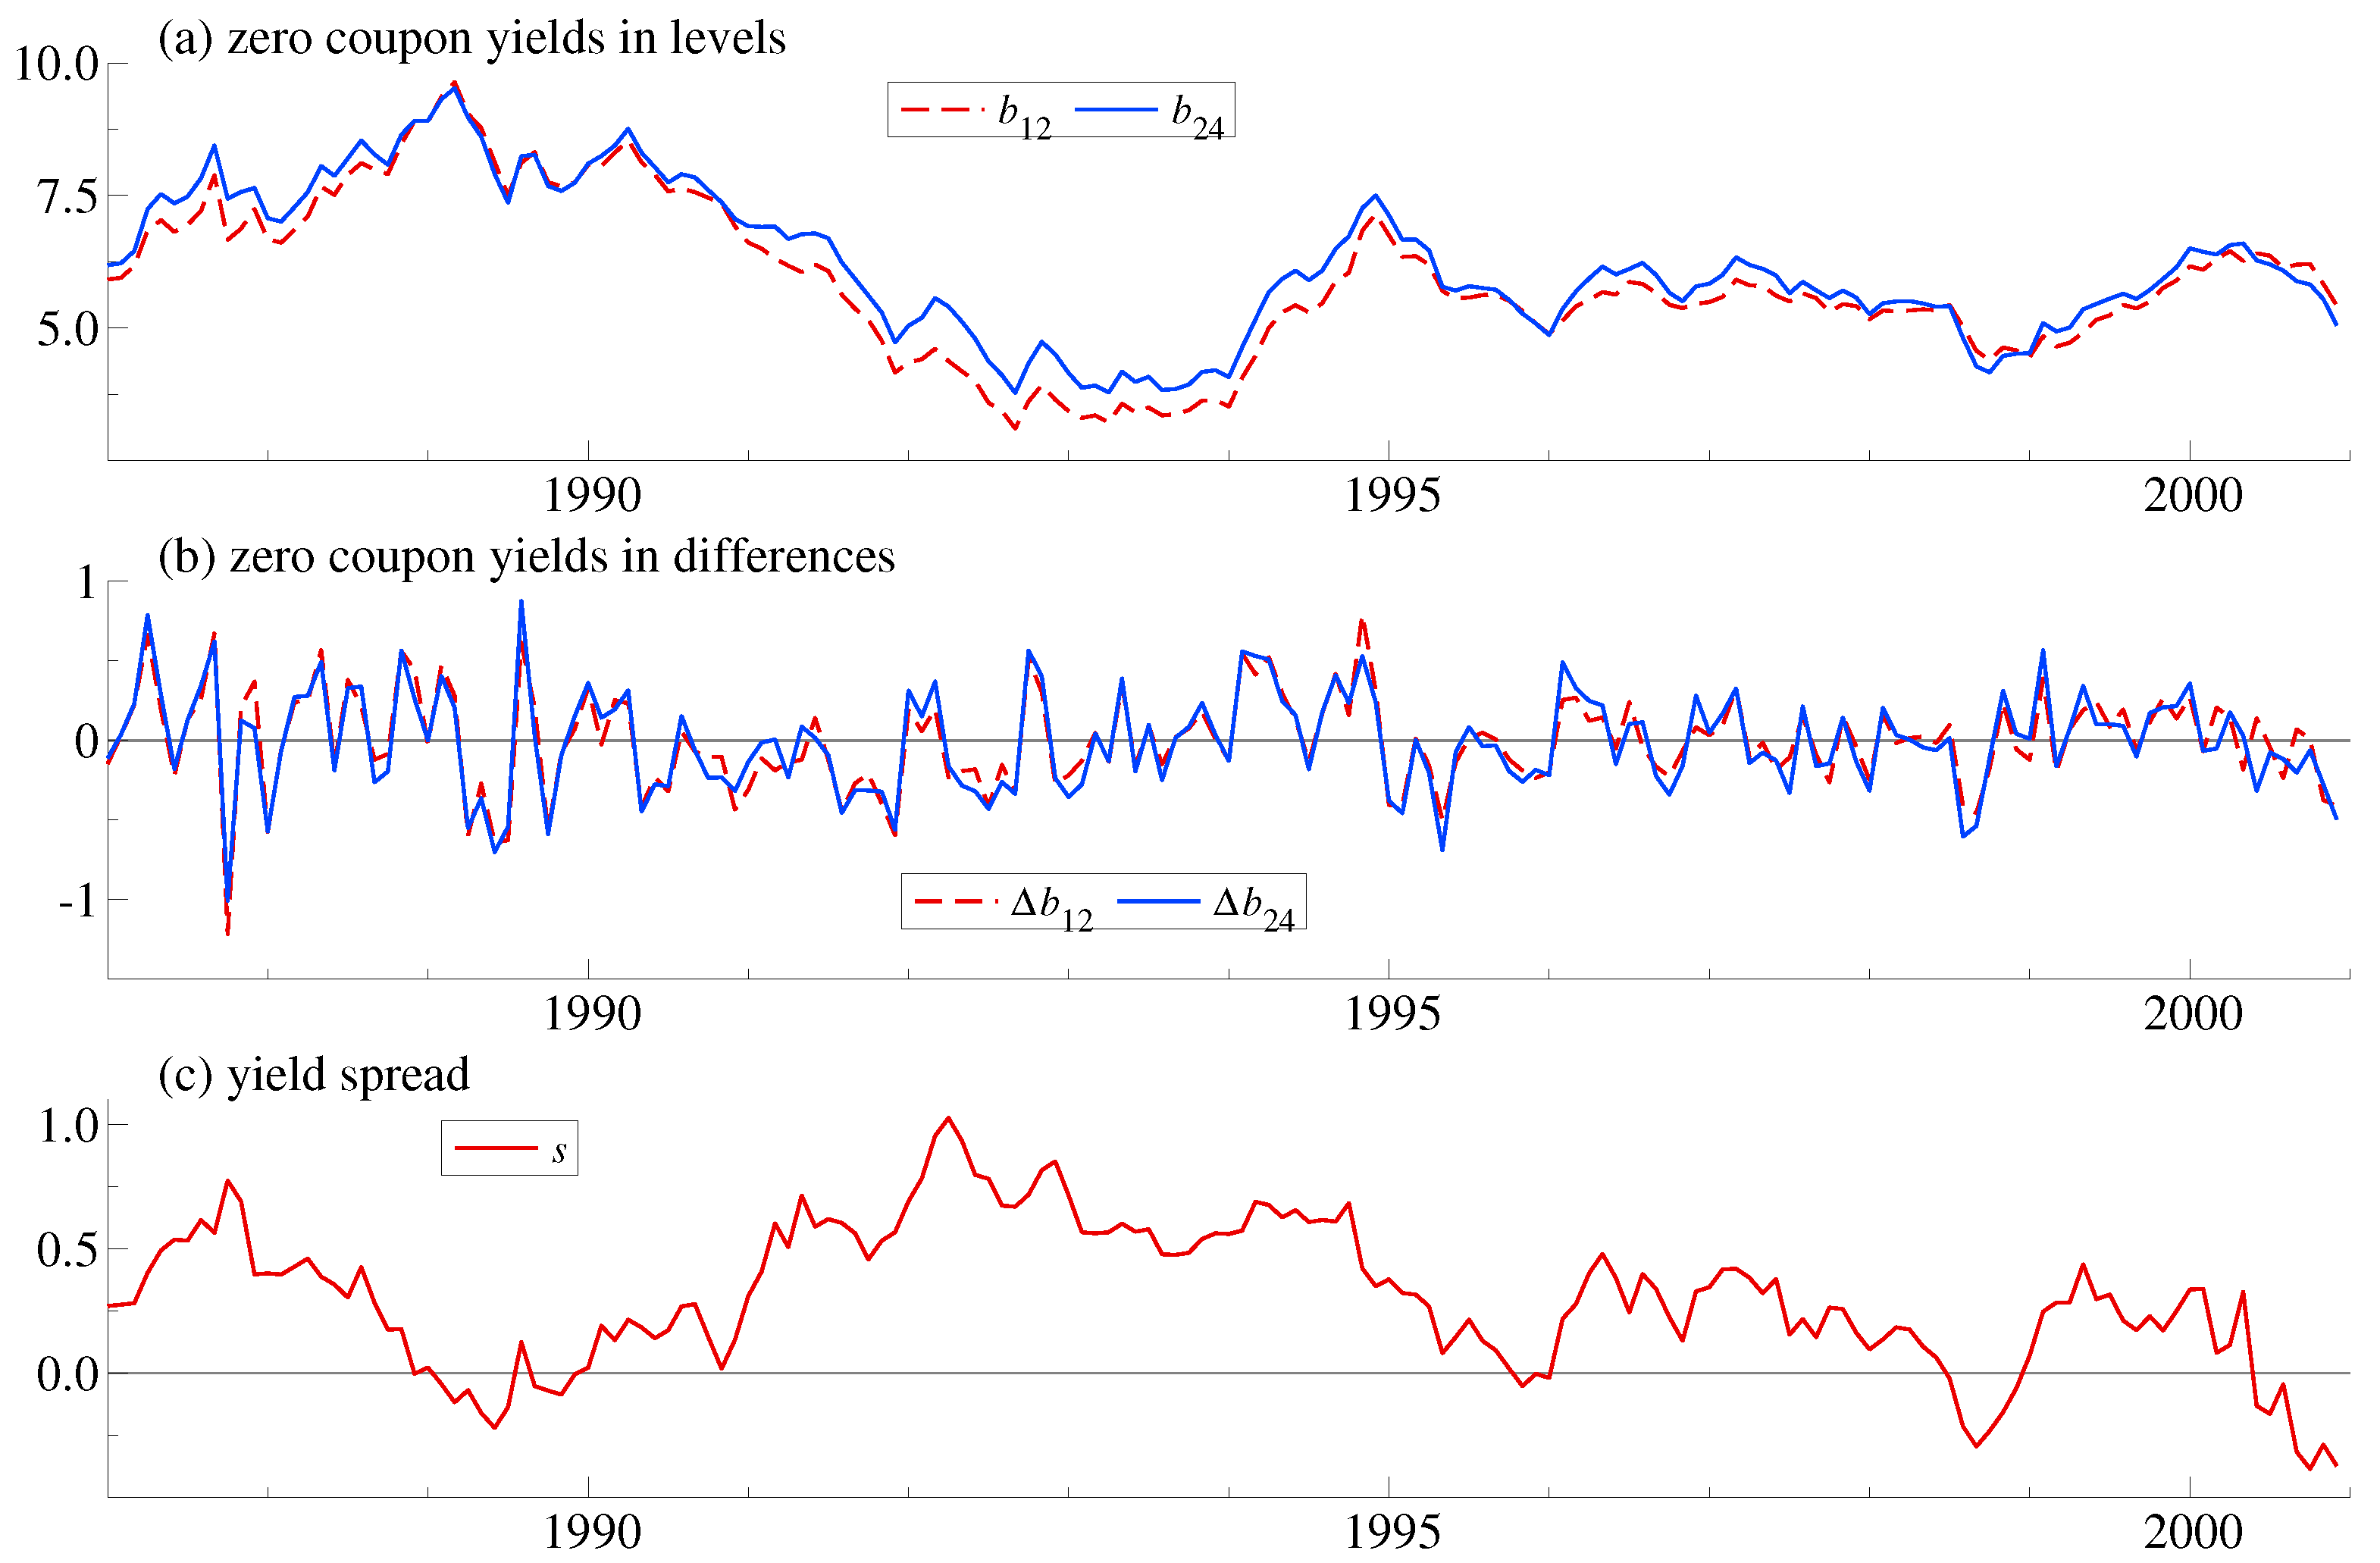
\includegraphics[width=1\linewidth]{coint1.png}
\end{figure}
    
\end{frame}





\begin{frame}{Examples}

    \textbf{1) Term structure of interest rates (yield curve)}
\[
i^{\text{long}}_t - \beta\, i^{\text{short}}_t \;\text{is stationary}
\]
Long and short rates move together in the long run (expectations hypothesis).
    \begin{figure}
        \centering
        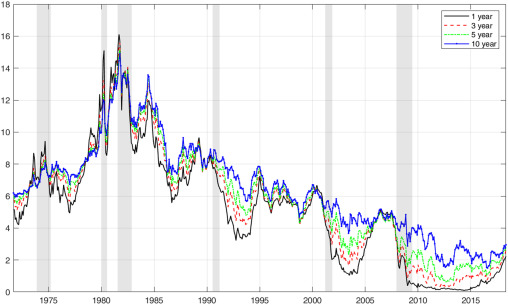
\includegraphics[width=0.75\linewidth]{coint yield curve.png}
    \end{figure}
\end{frame}



\begin{frame}{Examples}
\textbf{2) Exchange rate and relative prices (PPP)}
\[
e_t + p_t - p^{*}_t \;\text{is stationary}
\]
Nominal exchange rate and relative price levels co-move in the long run. \footnotesize (If domestic inflation: $\uparrow M, \downarrow X$, so nominal depreciation to compensate).

\begin{figure}
    \centering
    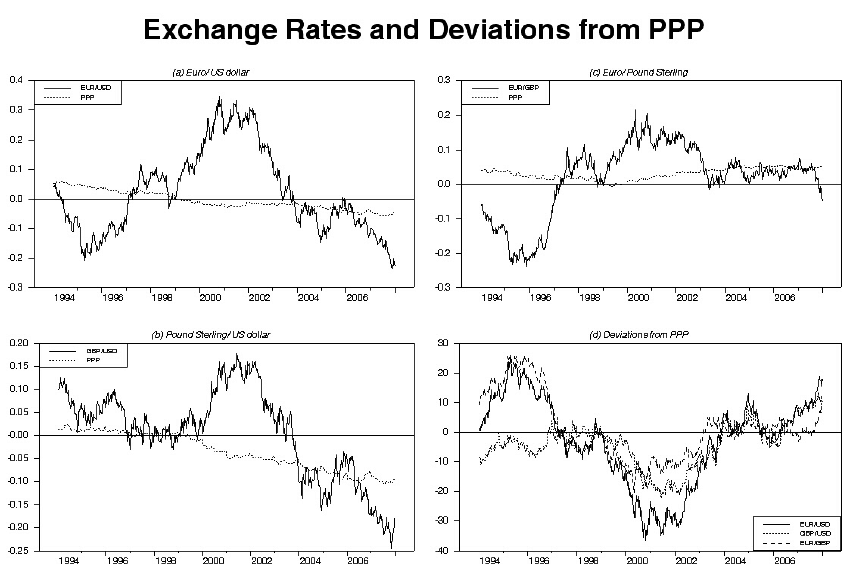
\includegraphics[width=0.75\linewidth]{PPP coint.png}
\end{figure}

\end{frame}



\begin{frame}{Examples}
\textbf{3) External constraint / Thirlwall's law}
\[
X_t - \beta_1 M_t - \beta_2 Y_t - \beta_3 Y^{*}_t \;\text{is stationary}
\]
Exports, imports, domestic and foreign income tied by the BoP constraint. The long-run growth rate of a country can be approximated by
\[
g \approx \frac{\text{growth of exports}}{\text{income elasticity of imports}}
\]
\footnotesize (If a country's income grows and it begins to import increasingly more, but its exports do not grow fast enough to pay for those imports, the country hits an external constraint and must slow down its growth.)


\end{frame}

\begin{frame}{Examples}

\textbf{4) Housing markets}
\[
P^{\text{house}}_t - \theta_1 R_t - \theta_2 Y_t \;\text{is stationary}
\]
House prices, rents and income linked by long-run affordability. Still the case? 

\begin{figure}
    \centering
    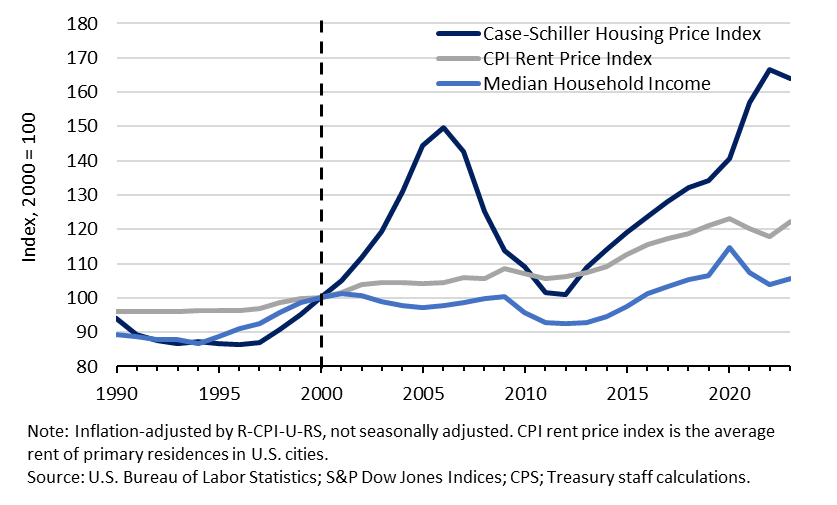
\includegraphics[width=0.75\linewidth]{price house rent.png}
\end{figure}

\medskip

\end{frame}

\begin{frame}{Examples}
\footnotesize
\textbf{5) Stock prices and dividends (Dividend discount model, empirically fragile)}
\[
P_t - \phi\, D_t \;\text{stationary?}
\]
Theory: prices and dividends are cointegrated. Prices correspond to dividends and expected returns. Dividends have a unit root, but expected returns are stationary. Over the long run prices will not deviate far from dividends. So 100\% of long-enough run price variation must come from dividend variation, not expected returns. But a more and more unstable relation (buybacks, QE, time-varying discount rates).
\begin{figure}
    \centering
    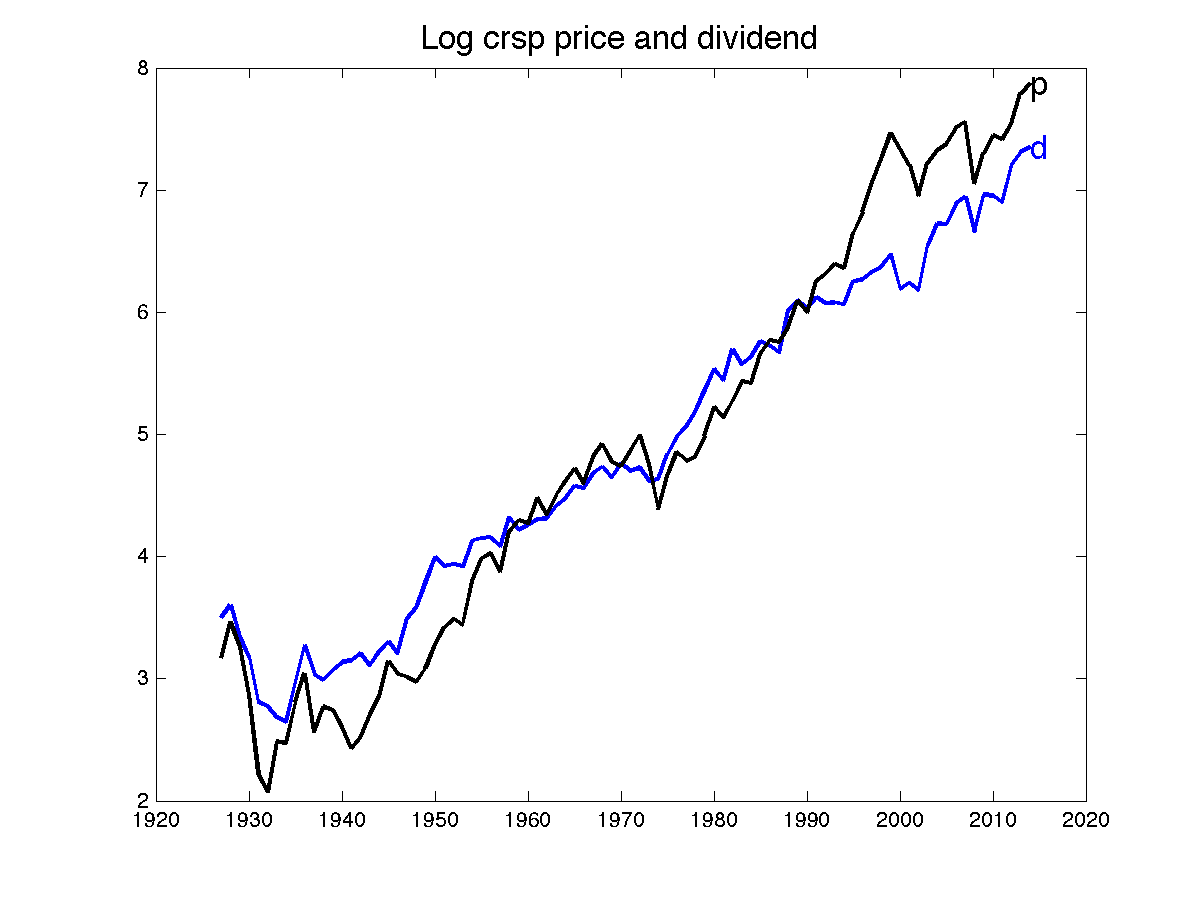
\includegraphics[width=0.55\linewidth]{divi coint.png}
\end{figure}

\end{frame}


\section{VECM}

%======================================================
\begin{frame}{Error-Correction Model (ECM)}
%======================================================
\small
Start with a bivariate long-run relation:
\[
y_t = \gamma_0 + \gamma_1 y_{t-1} + \gamma_2 x_{t-1} + u_t
\]
with $y_t, x_t \sim I(1)$ \textbf{AND} cointegrated.

Subtract $y_{t-1}$ (first-difference):
\[
\Delta y_t = \gamma_0 + (\gamma_1 - 1)y_{t-1} + \gamma_2 x_{t-1} + u_t
\]

Rearrange:
\[
\Delta y_t = \gamma_0 - \alpha \underbrace{(y_{t-1} - \beta x_{t-1})}_{\text{error-correction term}}
 + u_t
\]

\medskip
\textbf{Interpretation:}
\begin{itemize}
  \item $e_{t-1}=(y_{t-1} - \beta x_{t-1})$ = last period's deviation from long-run equilibrium (since, if stationary, then $\mathbb{E}(e_{t-1}) = 0$).
  \item $-\alpha$ = \textbf{speed of adjustment} back to equilibrium.\footnote{\footnotesize To make this factorisation work, we choose \(\alpha = 1 - \gamma_{1}\) and $\beta = \frac{\gamma_{2}}{1 - \gamma_{1}}$.}
\end{itemize}
\end{frame}

%======================================================
\begin{frame}{Interpretation of Error-Correction}
%======================================================
\small

\begin{itemize}


  \item If the error-correction term $e_{t-1} > 0$ (i.e.\ $y_{t-1}$ is \textbf{too high} relative to $x_{t-1}$), then:
  \[
  -\alpha e_{t-1} < 0 \quad \Rightarrow \quad \Delta y_t < 0
  \]
i.e.  $y_t$ is pushed downward in the next period. And conversely (if $e_{t-1} < 0$ (i.e.\ $y_{t-1}$ is \textbf{too low}, then $y_t$ is pushed upward.
\end{itemize}

\bigskip
The coefficient $-\alpha$ ($\alpha>0$) induces a  \textbf{systematic force that pulls $y_t$ back toward the long-run equilibrium relationship}.


\end{frame}


%======================================================
\begin{frame}{VECM Structure: Long-Run vs Short-Run}
%======================================================
\small
For $y_t$ a $k \times 1$ vector of $I(1)$ variables, the VECM (Vector ECM) of order $p$ - also called Johansen's model - is:
\[
\Delta y_t = \Pi y_{t-1}
 + \Gamma_1 \Delta y_{t-1}
 + \dots 
 + \Gamma_{p-1} \Delta y_{t-p+1}
 + u_t
\]
with
\[
\Pi = \alpha \beta',\quad
\beta: k\times r,\quad
\alpha: k\times r
\]

\begin{itemize}
  \item \textbf{$\beta'$ $y_{t-1}$}: $r$ long-run equilibrium relations (cointegrating combinations).
  \item \textbf{$\alpha$}: \textbf{adjustment (loading) coefficients} - how each variable reacts to short-run deviations from each equilibrium.
  \item \textbf{$\Gamma_i$}: short-run dynamics in differences (as soon as lags $p\geq2$).
\end{itemize}

\end{frame}




%======================================================
\begin{frame}{Cointegration rank and modelling choices}
%======================================================
\small
So the matrix $\Pi=\alpha\beta'$ captures the long-run structure. Its \textbf{rank} $r = \mathrm{rank}(\Pi)$ tells us how many \textbf{independent long-run equilibrium relations} exist among the $k$ variables, and how many \textbf{common stochastic trends remain.}

\begin{description}
  \item[$r = 0$:] \textbf{No cointegration}: 
    \begin{itemize}
      \item No stationary linear combination of $y_t$.
      \item \textbf{Model in differences:} VAR in $\Delta y_t$ (no error-correction term).
    \end{itemize}
  \item[$0 < r < k$:] \textbf{Cointegration present:}
    \begin{itemize}
      \item There are $r$ long-run relations, and $k-r$ stochastic trends.
      \item Use a\textbf{ VECM} with $\Pi = \alpha\beta'$:
      \begin{itemize}
           \item $\beta$ contains the $r$ cointegrating vectors;
          \item $\alpha$ contains the $k$ adjustment (loading) coefficients.
        \end{itemize}
    \end{itemize}
  \item[$r = k$:] All variables are effectively $I(0)$ (no unit root / RW):
    \begin{itemize}
      \item \textbf{Standard VAR in levels} on $y_t$ is appropriate, no need for first-differencing. 
    \end{itemize}
\end{description}
\end{frame}

%======================================================
\begin{frame}{What does the cointegration rank $r$ mean?}
%======================================================
\small
Example for a 3-variable system: $y_t = (y_{1,t}, y_{2,t}, y_{3,t})'$

\begin{description}
  % ---------- r = 1 ----------
  \item[$r = 1$:] only one stationary long-run relation (one correction term):
        \[
          \beta_1' y_t = b_{11} y_{1,t} + b_{21} y_{2,t} + b_{31} y_{3,t} \sim I(0)
        \]

So still two stochastic trends. 
  % ---------- r = 2 ----------
  \item[$r = 2$:] two independent stationary long-run relations, so still one stochastic trend:
        \[
        \beta_1' y_t =
          b_{11} y_{1,t} + b_{21} y_{2,t} + b_{31} y_{3,t} \sim I(0)
        \]
        \[
        \beta_2' y_t =
          b_{12} y_{1,t} + b_{22} y_{2,t} + b_{32} y_{3,t} \sim I(0)
        \]
  % ---------- r = 3 ----------
  \item[$r = 3$:] three stationary relations imply all variables are stationary:
        \[
        y_{1,t},\; y_{2,t},\; y_{3,t} \sim I(0)
        \] 
\footnotesize{(since it spans the entire space, i.e. can solve the stationary combinations to express each variable as a stationary function of the others)}

\smallskip
No VECM needed $\Rightarrow$ standard VAR in levels.
\end{description}

\end{frame}



%======================================================
\begin{frame}{Testing for cointegration}
%======================================================
\small
\textbf{Problem:} To test cointegration, we need to test whether
\[
\beta' y_t \sim I(0)
\]
for \emph{some unknown} $\beta$, right?

\medskip
\begin{itemize}
  \item We cannot test all possible linear combinations by ADF/PP individually on the specific difference results $e_t$! (we have a life)
  \item Cointegration involves the \textbf{system} as a whole, not marginal series.
  \item Need a \textbf{multivariate} method to estimate both 
        the number of relations $r$ and the vectors $\beta$.
\end{itemize}

\medskip
\textbf{Solution: Johansen (1988, 1991)} a full‐system maximum likelihood approach to cointegration.
\end{frame}


%======================================================
\begin{frame}{Johansen test}
%======================================================
\footnotesize

\textbf{Goal:} determine the \emph{cointegration rank} $r$, i.e.\ how many stationary long-run relations $\beta'y_t$ exist among $k$ $I(1)$ variables.

\medskip

\begin{itemize}
  \item Remember that $\Pi$ contains all \textbf{long-run} information.
  \item Johansen estimates its eigenvalues $\lambda_1 \ge \cdots \ge \lambda_k$ 
        measuring the "strength" of long-run relations.
  \item Large $\lambda_i$ $\Rightarrow$ one more cointegrating vector (i.e.  (deviations from the long-run combination are pulled back strongly); $\quad$ tiny $\lambda_i$ $\Rightarrow$ no further cointegration
\end{itemize}

\medskip

\textbf{Two statistics based on these eigenvalues:}
\begin{itemize}
  \item \textbf{Trace test:} tests $H_0: r \le r_0$ vs $H_1: r > r_0$:\quad $\lambda_{\mathrm{trace}}(r_0)=-T\displaystyle\sum_{i=r_0+1}^{k}\ln(1-\hat{\lambda}_i)$
  \item \textbf{Max-eigenvalue test:} tests $H_0: r=r_0$ vs $H_1: r=r_0+1$:\quad $\lambda_{\max}(r_0)=-T\ln(1-\hat{\lambda}_{r_0+1})$
  \end{itemize}
\medskip

\textbf{Procedure:} start from $r_0=0$ and \textbf{increase until tests fail to reject (increasing try-and-retry)}. The final $r$ is the estimated number of long-run equilibria.
\end{frame}



%======================================================
\begin{frame}{Practical Workflow with I(1) Variables}
%======================================================
\small
\begin{enumerate}
  \item \textbf{Unit root tests} on each variable ($I(0)$ vs $I(1)$).
  \item If all are $I(0)$: estimate a VAR in levels.
  \item If some are $I(1)$:
    \begin{itemize}
      \item Test for \textbf{cointegration rank $r$} (Johansen trace / max tests).
    \end{itemize}
  \item If $r = 0$: VAR in differences (short-run only).
  \item If $0 < r < k$: estimate a \textbf{VECM}, then:
    \begin{itemize}
      \item Interpret $\beta$ (long-run relations).
      \item Interpret $\alpha$ (who adjusts to what).
      \item Recover IRFs and FEVDs (via equivalent VAR in levels).
    \end{itemize}
\end{enumerate}

\textbf{NB:} you can of course have $I(0)$ variables alongside $I(1)$ ones (but they won't participate to cointegration so they will reduce the rank $r$ i.e. the number of long-term eq. relations). 

\end{frame}


%======================================================
\begin{frame}{Interpreting $\beta$ (long-run equilibrium) and $\alpha$ (adjustment)}
%======================================================
\footnotesize
% ------------------------ BETA ------------------------
\textbf{1) The cointegrating vector $\beta$ (long-run equilibrium)}
\begin{itemize}
  \item $\beta$ defines the \textbf{stationary long-run relation}.  
        Example: $C_t - 0.85\,Y_t$ stationary $\Rightarrow$ consumption-income move together.
        \item   Tells you \textbf{the fixed proportion} in which variables move together
        in the long run.
  \item Signs and ratios in $\beta$ describe \textbf{how variables co-move} in equilibrium.
  \item Only \textbf{relative coefficients} matter! Example of an estimated vector:
    \[
        \beta = (1,\,-2) \quad \Rightarrow \quad p_t - 2\,c_t \sim I(0)
        \]
        This means \textbf{in the long run, $p_t$ must be roughly twice $c_t$ (a 2:1 ratio)}.

        
        If $c_t$ increases by 1 point, staying on the long-run path requires  
        \[
        \Delta p_t = 2.
        \]
        If $c_t$ increases by 0.5, equilibrium requires  
        \[
        \Delta p_t = 1.
        \]
  \item \textbf{NB 1: if 3 variables and $r=1$} i.e. just one cointegration relation: β only gives the \textbf{equilibrium proportion, not who adjusts to  restor the ratio!}
  \item NB 2: if $\beta_i=0$,  plays \textbf{no role in the long-run equilibrium}, even if it is $I(1)$ (can still appear in $\Gamma$ as $\Delta$, but no in the cointegration space. \textbf{"Long-run exclusion"}).
\end{itemize}
\end{frame}


%======================================================
\begin{frame}{Interpreting $\beta$ (long-run equilibrium) and $\alpha$ (adjustment)}
%======================================================
\footnotesize


\textbf{2) The loading matrix $\alpha$ (error-correction / adjustment)}
\begin{itemize}
  \item $\alpha_i$ shows how variable $i$ reacts when the system deviates from equilibrium.
  \item $\alpha_i < 0$: variable $i$ \textbf{falls} to correct a positive disequilibrium.  
  \item $\alpha_i > 0$: variable $i$ \textbf{rises} to correct the disequilibrium.
  \item $\alpha_i = 0$: variable $i$ does \textbf{not adjust} $\Longrightarrow$ \textbf{weakly exogenous} for the long run.
  \item Large $|\alpha_i|$ $\Rightarrow$ \textbf{fast} adjustment.
\end{itemize}
\textbf{Examples:}
\begin{itemize}
  \item Prices adjust to costs, not the reverse: $\alpha_{\text{price}} > 0$, $\alpha_{\text{cost}} \approx 0$. Costs are weakly exogenous for the long run. 
\end{itemize}

\medskip
\textbf{3) The three restrictions that can occur in a VECM:}
\begin{itemize}
  \item \textbf{Weak exogeneity ($\alpha$-restriction):} $\alpha_i = 0$ $\Rightarrow$ variable $i$ does not adjust to long-run disequilibrium.
  \item \textbf{Long-run exclusion ($\beta$-restriction):} $\beta_i = 0$ in all cointegrating vectors $\Rightarrow$ variable $i$ does not enter the long-run equilibrium relation.
  \item \textbf{Short-run exclusion / Granger non-causality ($\Gamma$-restriction):} relevant row/column of $\Gamma$ is zero $\Rightarrow$ variable $i$ does not affect others in the \textbf{short-run dynamics}.
\end{itemize}
\end{frame}

%======================================================
\begin{frame}{Variables in $\beta$ but Weakly Exogenous ($\alpha_i=0$)}
%======================================================
\footnotesize
If a variable is in the long-run relation ($\beta_i \neq 0$) but weakly exogenous ($\alpha_i = 0$), what does it mean? 
\pause

\textbf{It is part of the long-run equilibrium but does not adjust to it... Thus it acts as the long-run anchor!} \textbf{External determinant} of the long-run path. 

\medskip
\hrule
\medskip

\textbf{Examples of long-run anchors:}
\begin{itemize}
  \item \textbf{Foreign interest rate} in a small open economy:  
        enters UIP ($\beta\neq 0$) but does not react to domestic deviations ($\alpha = 0$). It is the domestic rate which adjusts through depreciation, K flights, bond yields and key rate increase.
  \item \textbf{World oil price} for energy-importing countries:  
        drives domestic costs ($\beta\neq 0$) but is unaffected by local imbalances.
  \item \textbf{Productivity trend} in long-run wage equations:  wages used to adjust to productivity ($\beta\neq 0$), productivity does not adjust ($\alpha=0$)\textbf{ (except if Kaldor-Verdoorn law through demand and increasing returns!)}
  \item \textbf{Foreign GDP} in export demand: determines long-run export volumes (and thus domestic growth if\textbf{ Thirlwall's law}), but foreign GDP does not adjust to home exports.
  \item \textbf{Potential output} in Phillips-curve systems: defines the long-run gap but does not move with short-run inflation/output imbalances.
\end{itemize}

\end{frame}


%======================================================
\begin{frame}{Correlation $\neq$ Cointegration}
%======================================================
\footnotesize

\textbf{Correlation (static co-movement)}: measures \textbf{linear association at a point in time}:
  \begin{itemize}
  \item Can be high simply because both series \textbf{trend over time}, even if
        there is \textbf{no economic relation} (spurious correlation).
  \item Ignores the \textbf{order of integration} and \textbf{long-run behaviour}.
\end{itemize}

\medskip
\textbf{Cointegration (long-run equilibrium)} is about \textbf{common stochastic trends}, not about
        contemporaneous covariation. Can be uncorrelated in the short run!

\medskip
\textbf{Why they are different}
\begin{itemize}
  \item Two unrelated random walks can have \textbf{high correlation} but
        \textbf{no cointegration} (both just trend upward).
  \item Two series can be \textbf{cointegrated} even if their short-run
        correlation is \textbf{weak}: they may wander in the short run but
        \textbf{cannot drift apart permanently}.
\end{itemize}

\medskip
\begin{itemize}
    \item Two \textbf{drunk walkers} (random walk, $I(1)$) may step in different directions each moment $\Rightarrow$ low (or zero) correlation. 
    \item But if they are connected by a rope, they cannot drift apart indefinitely $\Rightarrow$ their \emph{distance} is stationary.
\end{itemize}

\end{frame}




\section{Papers}

%======================================================
\begin{frame}{Growth is wage-led in the long run (Barrales-Ruiz et al., 2025)}
%======================================================
\small

\textbf{Research question:}  why did US long-run growth and the labor share decline \emph{together} since the 1970s? Is long-run growth \textbf{wage-led} or \textbf{profit-led}?

\medskip

\textbf{Data (US, 1948Q1-2023Q4):}  
Real GDP growth $g_t$, labor share $\psi_t$, unemployment $u_t$.

\medskip

\textbf{Method:}  
\begin{itemize}
  \item Estimate a \textbf{Time Varying Parameter–VECM with stochastic volatility}:
        \begin{itemize}
          \item TVP because the US since 1945 had very different eras (Golden age, neoliberalism, financialisation) but evolving very gradually.
          \item Long-run equilibrium of the form:
          \[
            g_t = B_{1,t}\psi_t + B_{3,t}u_t
          \]
        \end{itemize}
  \item Johansen logic applied in a Bayesian VECM.
\end{itemize}

\end{frame}



%======================================================
\begin{frame}{Growth is wage-led in the long run (Barrales-Ruiz et al., 2025)}
%======================================================
\small

\textbf{Key long-run coefficient:}
\[
B_{1,t} > 0 \quad \text{for most of 1948–2023}.
\]
\begin{itemize}
  \item A \textbf{1 p.p. fall in labor share} $\to$ \textbf{0.25-0.40 p.p. fall in long-run GDP growth}.
  \item Long-run US growth is \textbf{wage-led}.
  \item Effect disappears 1975-1995 (neoliberal transition, profit-led), reappears after mid-1990s.
\end{itemize}

\medskip

\textbf{Transmission channels (via two additional VECMs):}
\begin{itemize}
  \item $\psi_t \to$ \textbf{consumption growth}: strong, robust, cointegrated effect.
  \item $\psi_t \to$ \textbf{labor productivity}: positive but significant only post-2000.
\end{itemize}

\emph{Short-run profit-led, long-run wage-led}.  
Consumption channel dominates the induced-technical-change channel.
\end{frame}


%======================================================
\begin{frame}{Cointegration of output, capital, labor, and energy (Stresing et al., 2008)}
%======================================================
\small

\textbf{Research question:} do the production factors $(K,L,E)$ and output $Q$ form a \textbf{long-run equilibrium relation}?  If yes, does the cointegrating vector match the Cobb-Douglas elasticities?

\medskip

\textbf{Data:} Germany, Japan, USA (1960-1990s).  
Variables: $\ln Q_t$, $\ln K_t$, $\ln L_t$, $\ln E_t$.

\medskip

\textbf{Method:}
\begin{itemize}
  \item All series are $I(1)$ $\Rightarrow$ test cointegration of:
  \[
    u_t = \ln Q_t - \alpha\ln K_t - \beta\ln L_t - \gamma\ln E_t.
  \]
  \item Impose \textbf{Cobb-Douglas structure:}  
  \[
    \alpha,\beta,\gamma\ge 0,\qquad \alpha+\beta+\gamma=1
  \]
  \item Identify $(\alpha,\beta,\gamma)$ by:
  \begin{itemize}
      \item Engle-Granger tests on residual stationarity,  
      \item RSS and Durbin-Watson to pick best vector.
  \end{itemize}
\end{itemize}

Cointegration vector interpreted as \textbf{empirical output elasticities}, not \textbf{cost shares!} (Giraud \& Kahraman (2014) on cost share Theorem's failure).
\end{frame}


%======================================================
\begin{frame}{Cointegration of output, capital, labor, and energy (Stresing et al., 2008)}
%======================================================
\small

\begin{itemize}
  \item $(Q,K,L,E)$ are \textbf{cointegrated} for Germany and USA; weaker but present for Japan.
  \item Estimated long-run elasticities differ sharply from neoclassical predictions:
  \[
    \alpha_K \approx 0.4\!-\!0.6,\qquad
    \beta_L \approx 0.05\!-\!0.2,\qquad
    \gamma_E \approx 0.3\!-\!0.6
  \]
  $\Rightarrow$ \textbf{Energy elasticity is huge; labor elasticity is small than K one}.
\end{itemize}

\textbf{Implications:}
\begin{itemize}
  \item Supports heterodox production theory (LINEX, thermodynamic constraints).
  \item Challenges neoclassical "cost share = elasticity" assumption (cf. Giraud \& Kahraman, 2014).
  \item Explains the energy crises (1973, 1979) as productivity shocks:\textbf{ output is highly sensitive to energy vs. Shapiro \& Watson (1988) (and the whole RBC literature)} saying that half of output volatility is due to change in labour supply (the causality is reversed).
\end{itemize}
\end{frame}
















\section{DFM}


\begin{frame}
  \centering
  \vfill
  {\LARGE \textbf{Dynamic Factor Models and Factor-Augmented VAR (FAVAR)}}\\[0.4cm]
  \vfill
\end{frame}

%======================================================
\begin{frame}{Why do we need dynamic factor models?}
%======================================================
\small

\textbf{Modern macro-finance datasets} contain \textit{dozens} or \textit{hundreds} of indicators:
\begin{itemize}
  \item production, employment, sales, prices, wages, multisectors;
  \item credit, spreads, house prices, asset prices, equity indexes;
  \item surveys, confidence indicators, expectations.
\end{itemize}

\medskip
\textbf{Goal:} exploit all this information for analysis, forecasting, and structural work.

\medskip
\pause
\textbf{But... curse of dimensionality!!!}
\[
\text{VAR}(k,p) \text{ has } \; k^2 p \; \text{parameters.}
\]
Example: variables $k=20$, lags $p=4$ $\Rightarrow$ $1600$ parameters.

\medskip
\textbf{Conclusion:} \textbf{OUCH!}

\end{frame}




%======================================================
\begin{frame}{Most macroeconomic series move together}
%======================================================
\small

\textbf{Stylised fact:} many macro and financial variables co-move due to a few
underlying forces:
\begin{itemize}
  \item the domestic and global \textbf{business cycles};
  \item the domestic and global \textbf{financial cycles};
  \item inflation regimes, uncertainty cycles, market sentiments... but not a lot of other things.
\end{itemize}

\medskip
Even if, obviously, idiosyncratic components differ, \textbf{cross-sectional comovement is strong!}

\pause
\begin{block}{What's the core idea of DFM?}
If $N$ is large,\textbf{ most of the variance} of $x_{1t},\dots,x_{Nt}$ can be explained
by \textbf{a small number of\textit{ hidden drivers}}.
\end{block}

\medskip
\textbf{Goal of DFM:} extract these few latent common components.
\end{frame}



%======================================================
\begin{frame}{Idea: replace hundreds of observables with a few factors}
%======================================================
\small

Instead of modelling all the $x_t \in \mathbb{R}^N$ directly, assume:
\[
x_t = \Lambda f_t + e_t,
\qquad
(x_t \in \mathbb{R}^N,\;
f_t \in \mathbb{R}^r,\;
\Lambda \in \mathbb{R}^{N \times r},\;
e_t \in \mathbb{R}^N)
\]
with $N$ large and $r \ll N$.

\medskip

\begin{itemize}
  \item $f_t$ = $r\times 1$ vector of \textbf{latent factors} (e.g.\ business cycle, financial cycle), with $r \ll N$ (often $r = 1,\dots,4$).
  \item $\Lambda$ = matrix of \textbf{factor loadings} $\lambda_i$ linking each $x_{it}$ to each factor.
  \item $e_t$ = \textbf{idiosyncratic} noise (variable-specific component and measurement errors).
\end{itemize}

\pause
\textbf{Benefits:}
\begin{itemize}
  \item compress $N$ time series into $r$ factors;
  \item estimate dynamics on $f_t$ with a small VAR;
  \item recover the impact $f_t$ on each $x_{it}$ using its loadings $\lambda_i$.
\textbf{  \item So a LOW-DIMENSION REPRESENTATION, called  a "STATE-SPACE" model}.
\end{itemize}

\end{frame}



%======================================================
\begin{frame}{What are these factor models used for?}
%======================================================
\small

\textbf{1. Forecasting (large datasets)}
\begin{itemize}
  \item GDP, inflation, credit growth can be forecast using factors summarising 100+ variables: more information!
\end{itemize}

\textbf{2. Nowcasting} (Giannone, Reichlin \& Small, 2008)
\begin{itemize}
  \item  $=$ real-time estimation of the current state of the economy (e.g. GDP) before official institutional statistics are released.
  \item handle missing/late data releases via the state-space representation (Kalman filter updates factor using monthly indicators (IP, PMI, retail sales, credit...)). \hyperlink{MF}{\beamergotobutton{Mixed Frequencies}}
\end{itemize}


\textbf{3. Structural analysis (Factor-Augmented VAR - FAVAR)}
\begin{itemize}
  \item identify shocks in a VAR augmented with factors.
  \item observe responses of hundreds of series through factor loadings.
\end{itemize}

\textbf{4. Macro-financial cycle analysis} (Miranda-Agrippino \& Rey, 2021)
\begin{itemize}
  \item Uncover common global (or cross-country) factors to analyse spillovers, co-movements, systemic risk across a panel of countries/assets. 
\end{itemize}

\end{frame}


%======================================================
\begin{frame}{DFM pipeline in short}
%======================================================
\small

To solve the curse of dimensionality:
\begin{enumerate}
  \item \textbf{we represent} $x_{it}$ as driven by a small number of common factors.
  \item \textbf{we estimate} these factors using Principal Component Analysis - PCA (large-$N$ consistency washing out idiosyncratic errors), cf. the Bootcamp.
  \item \textbf{we model} factor dynamics with a small VAR (forecasting / analysis / identification).
  \item \textbf{we map} factor shocks back to all original series via loadings.
\end{enumerate}
\end{frame}







%======================================================
\begin{frame}{Approximate factor model}
%======================================================
\small

\textbf{Exact factor model} (textbook):
\[
e_{it} \text{ (idiosyncratic components) are cross-sectionally uncorrelated.}
\]

\medskip
\textbf{Approximate factor model} (macro/finance practice):
\begin{itemize}
  \item $e_{it}$ may be of course weakly correlated across $i$ and $t$ despite the common factors.
  \item but \textbf{DOMINANT cross-sectional dependence} comes from $f_t$.
  \item i.e. most of the \textbf{covariance} of $x_t$ across $i=1,\dots,N$ is driven by a small number of common factors $f_t$.
\end{itemize}

\medskip
This is what allows us to estimate the factor space consistently \textbf{when $N$ is large} (lots of variables).

\medskip

Typical asymptotics: \textbf{large $N$}, \textbf{moderate/large $T$}.

\end{frame}


%======================================================
\begin{frame}{Estimating the factors by PCA}
%======================================================
\small
See Appendix for details: 
\hyperlink{pca-algorithm}{\beamergotobutton{PCA Algorithm}}

\medskip
Let $X = [x_1, \dots, x_T]$ be the $N \times T$ data matrix.

\medskip
\textbf{Objective:} find low-dimensional $f_t$ and $\Lambda$ such that
\[
x_t \approx \Lambda f_t
\]
for all $t$, i.e.\ minimise the \textbf{sum of squared idiosyncratic components}:
\[
\min_{\Lambda, (f_t)} \frac{1}{NT} \sum_{t=1}^T \| x_t - \Lambda f_t \|^2
\]
subject to a normalisation on $(f_t)$.

This is what \textbf{Principal Component Analysis (PCA)} does!
\begin{itemize}
  \item choose $r$ linear combinations of $x_t$ that \textbf{maximise explained variance} $\Rightarrow$ these are the \textbf{estimated factors}.
\end{itemize}

\medskip
$f_t$ are the \textbf{latent components} that best summarise all series.

\end{frame}





%======================================================
\begin{frame}{Why PCA?}
%======================================================
\small

PCA chooses $\hat{f}_t$ and $\hat{\Lambda}$ such that:
\begin{itemize}
  \item the first factor explains as much variance of $x_t$ as possible;
  \item the second factor explains as much as possible of the remaining variance;
  \item etc. with\textbf{ factors orthogonal to each other.}
\end{itemize}

\medskip
\begin{itemize}
  \item Hence the first few factors capture the \textbf{main comovements} in the data;
  \item idiosyncratic components $e_{it}$ absorb residual, variable-specific noise.
\end{itemize}

\end{frame}












%======================================================
\begin{frame}{From static to dynamic factors}
%======================================================
\small

\textbf{So far:} Static factor model, i.e. $f_t$ captures \textbf{cross-sectional comovement (only} at each $t$: $x_t = \Lambda f_t + e_t$

\medskip

\textbf{But macroeconomic and financial variables are dynamic.}

\begin{itemize}
  \item No distinction between contemporaneous factors vs. dynamic latent "forces" over time.
  \item Here we cannot model how shocks today affect future factors. 
  \item No factor autocorrelation structure, while factors themselves may be persistent.
  \item No lag structure between variables (what if employment lags industrial production by 4 months, or if housing leads the cycle?)
  \item For forecasting or structural analysis, we need a \textbf{law of motion} for $f_t$.
\end{itemize}

\medskip
This leads to the \textbf{Dynamic Factor Model (DFM)}.

\end{frame}


%======================================================
\begin{frame}{Dynamic Factor Model \& State-Space Representation}
%======================================================
\small

A \textbf{Dynamic Factor Model (DFM)}, written as a classical \textbf{state-space representation}:

\medskip
\textbf{1) State (Transition) Equation} (the latent drivers):
\[
f_t = A_1 f_{t-1} + \cdots + A_p f_{t-p} + u_t
\]
where $u_t$ is white noise.

\medskip

\textbf{2) Measurement Equation} (observables):
\[
x_t = \Lambda f_t + e_t
\]
\begin{itemize}
  \item $f_t$ are low-dimensional latent states.
  \item $x_t$ are high-dimensional observables.
  \item $(e_t)$ are idiosyncratic noise (variable-specific components and measurement errors).
\end{itemize}

\medskip
Now, common forces have their own dynamics and persistence, and transmit shocks to all variables through the loadings $\Lambda$.

\end{frame}



%======================================================
\begin{frame}{Interpreting factors and loadings}
%======================================================
\small

Once factors $\hat{f}_t$ are estimated, check:

\begin{itemize}
    \item \textbf{Correlation with known macro series}, e.g. $ \hat{f}^{(1)}_t \;$ vs GDP growth, or credit spreads, or trade flows etc. 
\textbf{    \item Visual inspection: }do peaks/troughs coincide with recessions or crises?
    \item \textbf{Sign of loadings:}  $\lambda_{ik}$ determines whether series $i$ moves \textbf{with} or \textbf{against} the factor.
    \item \textbf{Magnitude:} large $|\lambda_{ik}|$: series $i$ is strongly driven by factor $k$. Factor $k$ can be interpreted using those high-loading series.
    \item Cross-section of $\lambda_i$ tells you \textbf{which economic block} a factor corresponds to (real activity, credit, confidence, prices, financial stress, \dots)
    \end{itemize}

\medskip
\textbf{Interpretation is IMPORTANT: a factor must correspond to an economically meaningful latent force.}
\end{frame}



%======================================================
\begin{frame}{Robustness}
%======================================================
\small

\textbf{Number of factors:} in practice, the "true" $r$ is unknown.

\medskip
\begin{itemize}
  \item Look at the \textbf{proportion of variance explained} by the first $r$ components (e.g. if factor 1 $=75\%,$, factor 2 $=15\%$, factor 3 $=3\%$, maybe keep $r=2$).  
  \item Use the Bai-Ng \textbf{information criteria} ($IC(r)$ and $PC(r)$) minimisation for both static and dynamic factors.\footnote{ For DFM, you can compare with Hallin \& Liška's (2007) spectral-density test.}
\end{itemize}

In practice, do not obsess about whether $r = 2$ or $r = 3$, check \textbf{robustness}, i.e. if results change drastically when moving from $r=2$ to $r=3$, your empirical conclusions are fragile. 

\medskip

\textbf{Sensitivity to the dataset: }try also alternative subsets of variables (e.g.\ only real indicators, only financial indicators), different transformations (levels, growth rates, logs), and if sensitive to sample splits or sub-periods.


\medskip

\textbf{Interpretability:} look also at the loadings on the $x_{i,t}$. Do the loadings make economic sense?Are the factors stable over time? And again, think about the interpretation of each factor (e.g. trade cycle, credit cycle, etc). 

\end{frame}





%======================================================
\begin{frame}{Two-step estimation (Stock-Watson)}
%======================================================
\small
First method:

\medskip
\textbf{Step 1: Estimate static factors by PCA (the "initialisation")} \hyperlink{pca-algorithm}{\beamergotobutton{PCA Algorithm}}
\[
\hat{f}_t = V_r' x_t,
\qquad
\hat{\Lambda} = \frac{1}{T} X \hat{F}'
\]

\medskip

\textbf{Step 2: Estimate dynamics via VAR}
\[
\hat{f}_t = \hat{A}_1 \hat{f}_{t-1} + \cdots + \hat{A}_p \hat{f}_{t-p} + \hat{u}_t
\]

\begin{itemize}
  \item Simple, fast, works well when $N$ is large.
  \item Consistent estimation of factor space as $N \to \infty$.
  \item Easy to implement for forecasting or FAVAR.
  \item \textbf{BUT } does not optimally handle missing data or small $N$ ($N<20$:\textbf{ PCA unreliable!)}
\end{itemize}
\end{frame}

%======================================================
\begin{frame}{Kalman Filter + EM Estimation}
%======================================================
\small

Using the state-space form, one can estimate $(f_t, A_i, \Lambda)$ jointly via:

\begin{itemize}
  \item \textbf{Kalman Filter + Smoother} \hyperlink{kalman-intuition}{\beamergotobutton{Kalman: intuition}}
  \item \textbf{EM algorithm} for maximum likelihood \hyperlink{em-intuition}{\beamergotobutton{EM: intuition}}
\end{itemize}
$\Rightarrow$
\begin{itemize}
  \item Handles \textbf{missing observations} efficiently.
  \item Especially useful when $N$ is \textbf{small or moderate}
  \item Allows \textbf{time-varying parameters} \textbf{(TVP-DFM).}
  \item Enables sophisticated applications such as nowcasting, mixed-frequency data (e.g. GDP in quarters, Prices in months).
\end{itemize}

\medskip
\scriptsize \textbf{NB}: Factors can even be estimated in the \textbf{frequency domain} (generalized DFM (GDFM) à la Forni et al. (2000), by spectral density: each factor contribution can be decomposed into medium-term (productivity/credit), business-cycle and high-frequency (financial stress) bands. E.g. one factor may dominate low frequencies, another one high ones.

\end{frame}





\section{FAVAR}

%======================================================
\begin{frame}{From DFMs to VARs: the FAVAR idea}
%======================================================
\small

Suppose we care about a small set of macro variables $(y_t,\; \pi_t,\; i_t)$ but we also observe a large information set 
\[
x_t = (x_{1t}, \dots, x_{Nt})',
\quad N \gg 3
\]

\medskip
How to incorporate the information in $x_t$ without estimating a huge VAR?

\bigskip
\textbf{Factor-Augmented VAR (FAVAR)} (Bernanke, Boivin \& Eliasz, 2005)
\begin{enumerate}
    \item Extract factors $\hat{f}_t$ from $x_t$ using PCA.
    \item Construct the augmented vector $   z_t = (y_t, \pi_t, i_t, \hat{f}_t)'$
    \item Estimate a small VAR in $z_t$.
\end{enumerate}

\medskip
So that we can use a \textbf{rich datasets} while keeping a \textbf{low-dimensional VAR}!

\medskip

Moreover, \textbf{more reliable identification!} Since\textbf{ factors absorb the omitted variables }that contaminate shocks.

\end{frame}

%======================================================
\begin{frame}{Impulse responses}
%======================================================
\footnotesize
Reduced-form forecasting and structural identification proceed exactly as in a usual SVAR (Cholesky, sign restrictions, narrative shocks etc.).

\medskip
\textbf{What changes:}
\begin{itemize}
  \item Now, the shock affects both observables $(y_t,\pi_t,i_t)$...
  \item And the latent factors $\hat{f}_t$ summarising $N$ other variables.
\end{itemize}

\medskip
\begin{itemize}
    \item  So 1) IRFs for $y_t$, $\pi_t$, $i_t$
    \item  But also 2) IRFs of the factors to structural shocks (their response)
    \item And then 3) map factor responses back to each of the $N$ variables ( \textbf{every $x_{it}$}, not in the VAR) via loadings $\hat{\Lambda}$:
\[
\widehat{\text{IRF}}_{x_{it}}(h)
    = \hat{\lambda}_i' \cdot \widehat{\text{IRF}}_{f}(h)
\]
\end{itemize}
Thus, one shock produces \textbf{impulse responses for all 100+ variables!} E.g. detailed policy transmission. 

\begin{itemize}
    \item Which factors react the most?
    \item Which variables are most sensitive to each factor?
    \item How fast do effects propagate and decay?
    \item Cycle propagation, foreign policy spillovers, financial amplification...
\end{itemize}
\end{frame}




%======================================================
\begin{frame}{Examples}
%======================================================
\scriptsize

Construct a business-cycle dataset with:
\begin{itemize}
    \item Industrial production,
    \item Hours worked and Employment
    \item Sales,
    \item Consumption indicators,
    \item Survey indices.
\end{itemize}
PCA typically extracts a first factor that tracks $\approx$ GDP growth.

\smallskip
Construct a financial dataset with:
\begin{itemize}
    \item Credit growth,
    \item Leverage,
    \item Corporate bond spreads,
    \item Equity prices,
    \item House prices,
    \item Volatility indices.
\end{itemize}
The first factor often captures the "financial cycle".

\medskip

Then MonPol shock in FAVAR: observe \textbf{how the cycle factors} respond, and then\textbf{ how each underlying series} responds. Examine whether the financial cycle \textbf{leads or lags} the business cycle.

\medskip
\textbf{NB:} thus, factors often track key macro series (same peaks and throughts, but \textbf{SMOOTHER} since less noise, being the "common signal"!)

\end{frame}











\section{Core example}


%======================================================
\begin{frame}{International Monetary Trilemma vs Rey's Dilemma}
%======================================================
\scriptsize

\textbf{Classical "Impossible Triangle" (Mundell-Fleming):}
\pause
\begin{itemize}
  \item Policy-makers can choose at most \textbf{two} of:
  \begin{itemize}
    \item Free capital mobility;
    \item Fixed (or tightly managed) exchange rate;
    \item Independent monetary policy.
  \end{itemize}
  \item With \textbf{free capital mobility}, the textbook recipe is:
  \begin{itemize}
    \item \emph{Fixed} FX $\Rightarrow$ no monetary autonomy (since CB must manage the FX)
    \item \emph{Floating} FX $\Rightarrow$ regain monetary autonomy (FX absorbs shocks)
  \end{itemize}
\end{itemize}
\begin{figure}
    \centering
    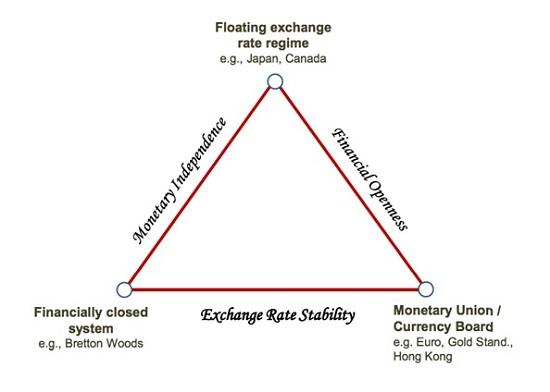
\includegraphics[width=0.55\linewidth]{Mundell tr.png}
\end{figure}

\end{frame}


%======================================================
\begin{frame}{Rey's "Dilemma" and the Global Financial Cycle}
%======================================================
\scriptsize

\textbf{Starting point:} the "Rey's Dilemma" (Rey, 2015) - the Global Financial Cycle (GFCy) undermines the classical trilemma.

\smallskip
\textbf{Miranda-Agrippino \& Rey (2015/2021, "(US Mon Pol \&) The Global Financial Cycle"):}
\begin{itemize}
  \item Provide a \textbf{systematic empirical measurement} of the GFCy;
  \item Quantify its importance in global risky asset prices, capital flows (FDI, portfolio, banking), private sector credit...
\end{itemize}

\textbf{Method: }
\begin{itemize}
  \item Build large panels: world risky asset returns (equity, credit, etc.); K flows (gross inflows/outflows by type) for $\sim$80 countries, 1990-2018; Credit and other macro-financial quantities.
  \item Estimate \textbf{DFM} - extract a \emph{global} factor and possibly group-specific factors for both prices and quantities.
  \item Study co-movements with \textbf{VIX and identified US monetary policy shocks}.
  \end{itemize}

\textbf{Main results:}
\begin{itemize}
  \item A small number of factors explain a \textbf{large share} of variation in risky asset prices and K flows $\Rightarrow$ strong, time-varying GFCy.
  \item US Mon Pol shocks significantly move the global factor
        ("center-country" channel).
        \item \textbf{Dilemma:} \textbf{with free capital mobility, \emph{floating FX is not enough} to ensure
        monetary independence. Need capital account control (directly via capital controls or indirectly via macroprudential tools)!}
  \item  \textbf{Heterogeneous} sensitivity: EMEs and financially open economies are more exposed!
  \item See Boyarchenko \& Elias (2024) on a decomposition of the GFCy into a \textit{Global Credit Cycle }and a \textit{Global Risk Factor}.
\end{itemize}

\end{frame}





%======================================================
\begin{frame}{Rey's "Dilemma" and the Global Financial Cycle}
%======================================================

\begin{figure}
    \centering
    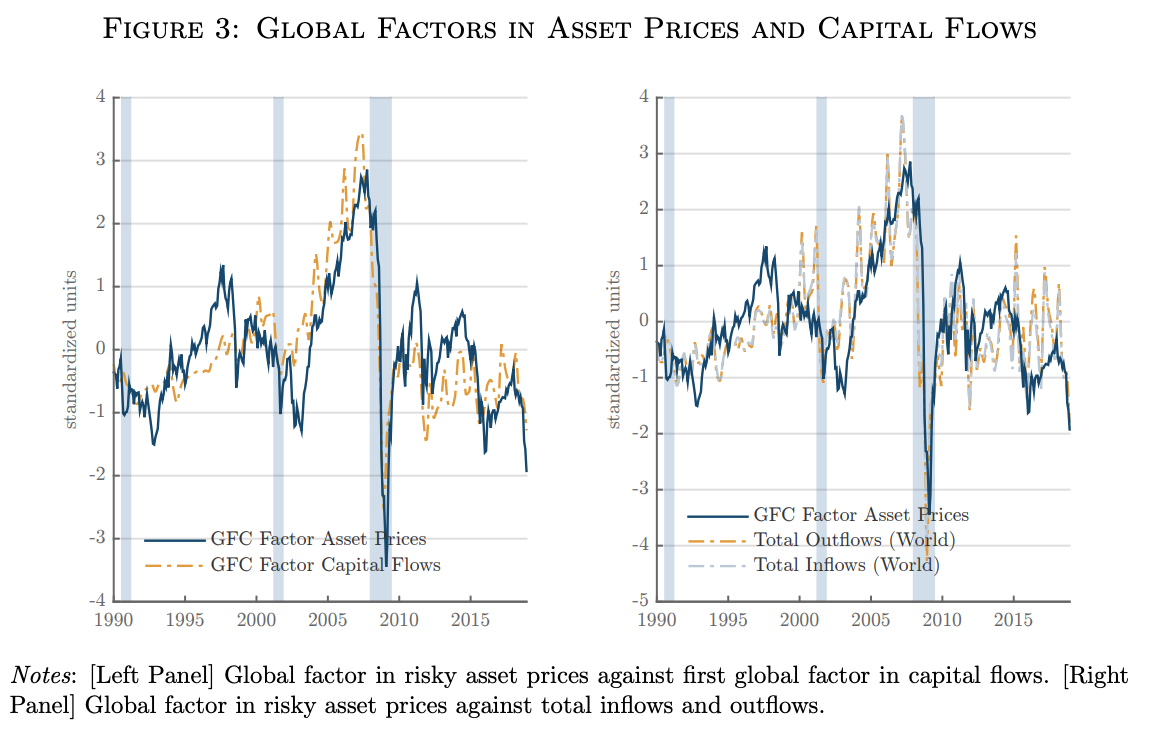
\includegraphics[width=1\linewidth]{global factor Rey.png}
\end{figure}
\end{frame}







%======================================================
\begin{frame}{Rey's "Dilemma" and the Global Financial Cycle}
%======================================================


\begin{figure}
    \centering
    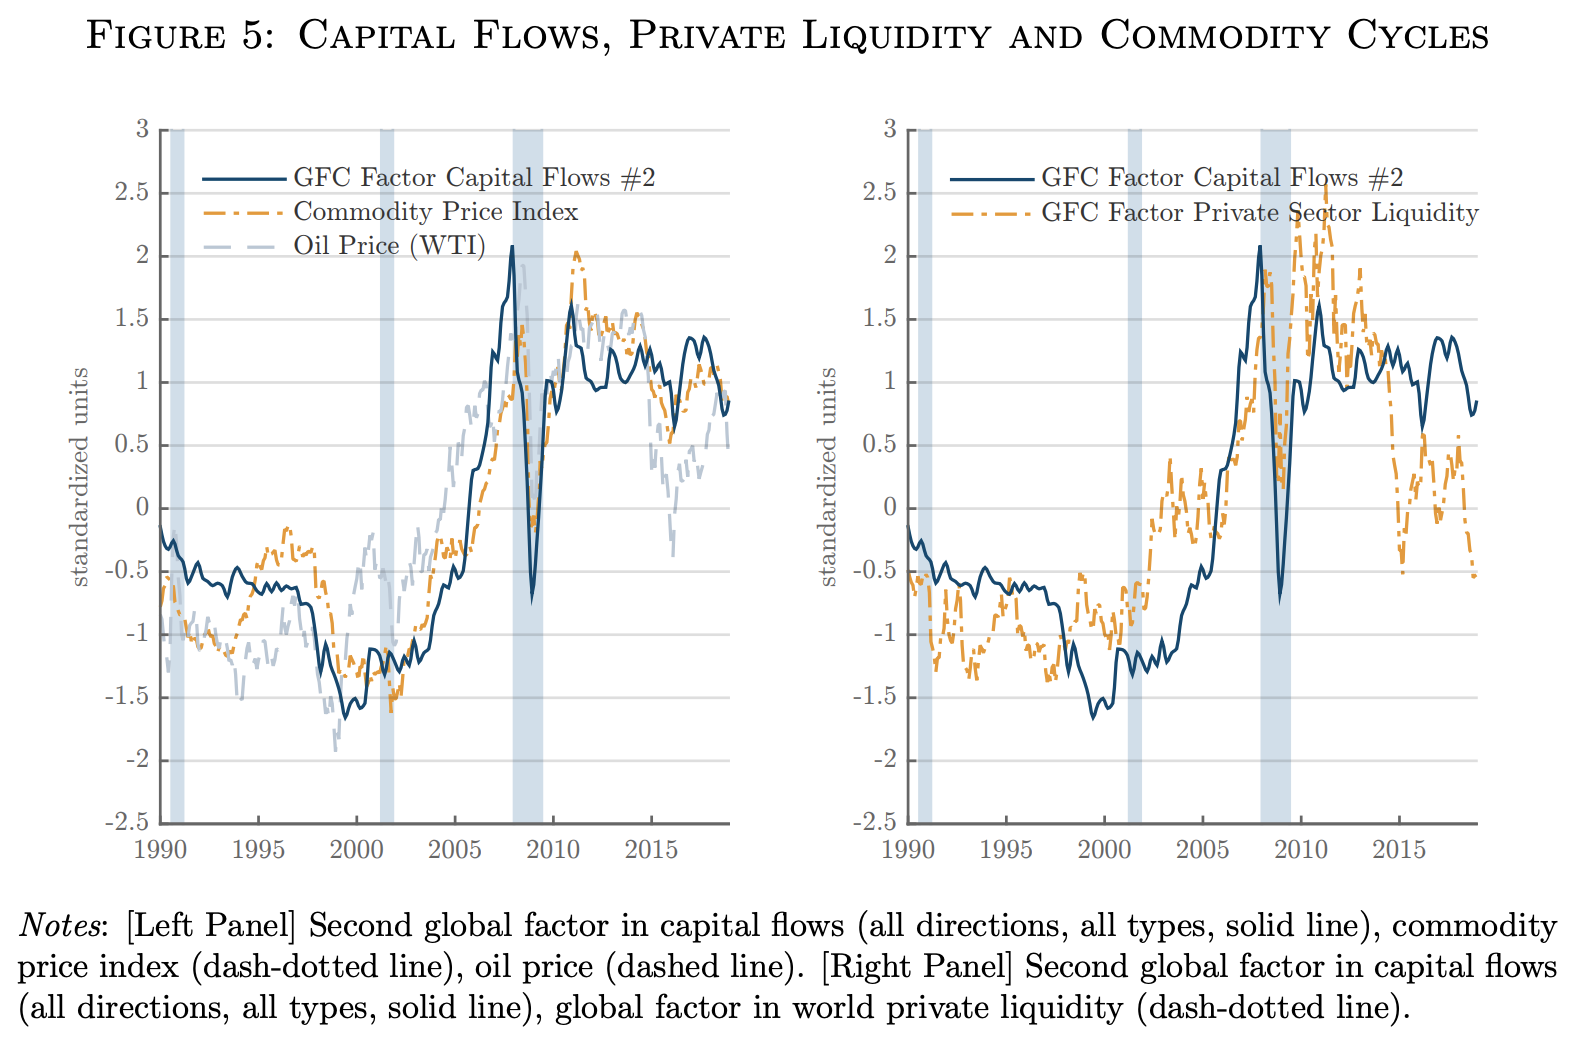
\includegraphics[width=1\linewidth]{Commod factor Rey.png}
\end{figure}

\end{frame}



\section{Appendix}

\begin{frame}
  \centering
  \vfill
  {\LARGE \textbf{Appendix}}\\[0.4cm]
  \vfill
\end{frame}

%======================================================
\begin{frame}{Regularization-based dimensionality reduction}
%======================================================
\footnotesize

Not all dimensionality reduction comes from latent factors. Sometimes we keep all variables but \textbf{shrink} coefficients.

\medskip

\textbf{1. Ridge regression}
\[
\min_\beta \|y - X\beta\|^2 + \lambda \|\beta\|^2
\]
\begin{itemize}
    \item Shrinks coefficients toward 0 (never exactly 0).
    \item Reduces variance, keeps all predictors.
    \item Good when predictors are highly correlated (“collinearity”).
\end{itemize}

\textbf{2. LASSO}
\[
\min_\beta \|y - X\beta\|^2 + \lambda \|\beta\|_1
\]
\begin{itemize}
    \item Performs \textbf{variable selection} (some $\beta_j = 0$).
    \item Reduces dimensionality by selecting a sparse subset of variables.
\end{itemize}

\textbf{3. Elastic net}
\[
\min_\beta \|y - X\beta\|^2 + 
\lambda\left( \alpha \|\beta\|_1 + (1-\alpha)\|\beta\|^2\right)
\]
\begin{itemize}
    \item Combines Ridge + LASSO.
    \item Useful when many predictors are correlated (macro/finance case).
\end{itemize}

\end{frame}



%======================================================
\begin{frame}[label=pca-algorithm]{Algorithm of the PCA estimator}
%======================================================
\small

\textbf{Step 1: Standardise each series}
\begin{itemize}
  \item For each $i$, subtract mean and divide by standard deviation of $x_{it}$.
\end{itemize}

\medskip
\textbf{Step 2: Sample covariance matrix}
\[
\hat{\Sigma}_x = \frac{1}{T} \sum_{t=1}^T x_t x_t' = \frac{1}{T} X X'
\]

\medskip
\textbf{Step 3: Principal components}
\begin{itemize}
  \item Compute eigenvalues/eigenvectors of $\hat{\Sigma}_x$.
  \item Let $V_r$ be the $N \times r$ matrix of eigenvectors associated with the
        $r$ largest eigenvalues.
\end{itemize}

\textbf{Estimated factors (at each $t$):} $\hat{f}_t = V_r' x_t$

\textbf{Estimated loadings:} $\hat{\Lambda} = \frac{1}{T} X \hat{F}'$ where $\hat{F} = [\hat{f}_1, \dots, \hat{f}_T]$ is $r \times T$

\end{frame}



%======================================================
\begin{frame}{Identification: rotation Invariance}
%======================================================
\small

Model:
\[
x_t = \Lambda f_t + e_t
\]

\textbf{Non-uniqueness issue} since for any invertible $H \in \mathbb{R}^{r \times r}$
\[
x_t = \underbrace{\Lambda H}_{\tilde{\Lambda}} \underbrace{H^{-1} f_t}_{\tilde{f}_t} + e_t
\]

\begin{itemize}
  \item $(\Lambda, f_t)$ and $(\tilde{\Lambda}, \tilde{f}_t)$ generate the same $x_t$.
  \item Only the \textbf{subspace spanned by the factors} is identified.
\end{itemize}

Thus we impose a \textbf{normalisation}, e.g.
\[
\frac{1}{T} \sum_{t=1}^T f_t f_t' = I_r
\qquad\text{and}\qquad
\Lambda'\Lambda \text{ diagonal}
\]


\end{frame}


%======================================================
\begin{frame}[label=kalman-intuition]{Kalman Filter + EM Estimation 1/2}
%======================================================
\scriptsize

\textbf{Goal:} given many \textbf{noisy} indicators $x_t$ (industrial production, surveys, spreads, \dots), recover the latent factors $f_t$ (``the common state of the economy'') in \textbf{real time}.

\medskip

\textbf{Kalman Filter = recursive "smart averaging" (precision-weighted average)}

\medskip

\underline{\textbf{1. Prediction step (before seeing $x_t$)}}  
\tiny
\[
\hat{f}_{t|t-1} = A\, \hat{f}_{t-1|t-1},
\qquad
P_{t|t-1} = A\, P_{t-1|t-1} A' + Q \text{ with } P_{t|t} = \operatorname{Var}(f_t - \hat{f}_{t|t})\]
\begin{itemize}
\tiny
  \item Predict the factor using its VAR dynamics.
  \item Predict its uncertainty ($P=$ covariance matrix of the estimation error of the state) : \textbf{uncertainty increases} because of the state shock $Q$.
  \item Intuition: this is the "model-based best guess" of the economy before seeing new data.
\end{itemize}

\medskip
\scriptsize
\underline{\textbf{2. Update step (after observing $x_t$)}}  
\tiny
\[
K_t = P_{t|t-1} \Lambda' (\Lambda P_{t|t-1} \Lambda' + R)^{-1}
\]
\[
\hat{f}_{t|t} = \hat{f}_{t|t-1} + K_t (x_t - \Lambda \hat{f}_{t|t-1})
\]
\[
P_{t|t} = (I - K_t \Lambda) P_{t|t-1}\]

\begin{itemize}
\tiny
  \item $K_t$ = \textbf{Kalman gain}: how much to trust the data vs. the prediction.
  \item If $R$ (measurement noise) is large $\Rightarrow$ trust the model more → small update.
  \item If prediction error $(x_t - \Lambda\hat{f}_{t|t-1})$ is large and reliable → strong correction.
  \item Posterior uncertainty $P_{t|t}$ shrinks when the new data are informative.
\end{itemize}

\medskip

\scriptsize
\textbf{Why it is powerful in DFM}
\begin{itemize}
\tiny
  \item Noisy series are automatically down-weighted (via $R$).  
  \item Missing data: simply omit the corresponding row of $\Lambda$ and $R$ in the update.  
  \item Under Gaussian assumptions: \textbf{optimal linear estimator} of $f_t$ at each $t$.
\end{itemize}

\end{frame}



%======================================================
\begin{frame}[label=em-intuition]{Kalman Filter + EM Estimation 2/2}
%======================================================
\scriptsize

\textbf{Problem:} the Kalman filter/smoother needs the parameters 
$\theta = (\Lambda, A_1,\dots,A_p,$ variances$)$.
How do we estimate $\theta$ by maximum likelihood when the factors $f_t$ are \emph{unobserved}?

\medskip

\textbf{Idea of EM = "fill in the factors, then re-estimate"}
\begin{itemize}
  \item Treat $f_t$ as \textbf{missing data}.
  \item Alternate two steps until convergence of the log-likelihood:
\end{itemize}

\medskip

\textbf{E-step (Expectation)}
\begin{itemize}
  \item Given a current guess of parameters $\theta^{(k)}$, run
        \textbf{Kalman Filter + Smoother} on the data.
  \item This gives the conditional expectations
        $\mathbb{E}[f_t \mid x_{1:T}, \theta^{(k)}]$ and
        $\mathbb{E}[f_t f_{t-1}' \mid x_{1:T}, \theta^{(k)}]$.
  \item Intuition: we "reconstruct" the latent factor paths as well as possible given $\theta^{(k)}$.
\end{itemize}

\medskip

\textbf{M-step (Maximization)}
\begin{itemize}
  \item Treat these reconstructed factors as known and re-estimate:
  \begin{itemize}
  \scriptsize
    \item \textbf{Loadings} $\Lambda$: regress $x_t$ on $f_t$ (cross-sectional regressions).
    \item \textbf{Dynamics} $(A_1,\dots,A_p)$: run a VAR on $f_t$.
    \item \textbf{Noise variances}: use residual variances from both steps.
  \end{itemize}
  \item This gives updated parameters $\theta^{(k+1)}$ that \textbf{increase} the likelihood.
\end{itemize}

\medskip


\begin{itemize}
  \item EM uses the Kalman smoother to "guess" the latent factors,
        then updates the parameters as if factors were observed.
  \item Repeat E- and M-steps until changes in $\theta$ or in the log-likelihood are very small.
  \item Result: Maximum Likelihood estimates of $(\Lambda, A_i,$ variances$)$ and smoothed factors $f_t$,
        well-suited for small $N$, missing data, and more complex DFMs.
\end{itemize}

\end{frame}



\begin{frame}[label=MF]{Mixed-frequency data}
\scriptsize
Some variables arrive \emph{often} (daily/weekly/monthly: rates, spreads, surveys...), while targets arrive \emph{rarely} (quarterly: GDP).

\medskip
\textbf{The temporal aggregation bias} (Working, 1960): if the true\textbf{ high-frequency process is dynamic} (e.g. AR), then time-aggregation (sum/average/end-of-period) :
\begin{itemize}
\item \textbf{alters the dynamics} (an AR at high frequency becomes \textbf{ARMA} at low frequency (serial correlation is created/reallocated)
\item \textbf{distorts timing and persistence} (intra-quarter shocks are smeared across the low-frequency periods $\Rightarrow$ spurious inertia and wrong lag structure)
\item \textbf{filters the spectrum} (aggregation behaves like a \textbf{low-pass filter} $\Rightarrow$ loss of within-quarter information)
\end{itemize}

\textbf{Two solutions keeping frequencies as they are : 1) DFM} (e.g. quarterly variables are \emph{observations of an aggregation} of\textbf{ latent} monthly states (handled naturally with missing data) $\Rightarrow$ Kalman filter/smoother. E.g.: $Y_T^{(Q)} = \lambda_Q \bigl( F_{3T} + F_{3T-1} + F_{3T-2} \bigr) + \varepsilon_T^{(Q)}$. \textbf{The latent factor must be specified at the highest available frequency.} But DFM = HUGE!

\medskip
\textbf{2) MIDAS (lightweight, reduced-form, forecasting-first)}: instead of aggregating $x$ into one quarterly number, regress the low-frequency target on \emph{many} high-frequency lags, but compress them with a smooth weighting function:
\[
y_T = \alpha + \beta \sum_{k=0}^{K} w(k;\theta)\, x_{T,k} + e_T,
\quad
\sum_{k=0}^K w(k;\theta)=1
\]
$\Longrightarrow$ learn a \textbf{distributed-lag profile} (recent lags matter more? Delayed peak? Hump-shaped?) with only a few parameters $\theta$.
\end{frame}



\end{document}

